\section{Performance Evaluation}\label{sec:evaluation}

\subsection{Methodology}

\begin{figure*}[t]
      \centering
      \vspace{-2pt}
        \subfigure[] {
        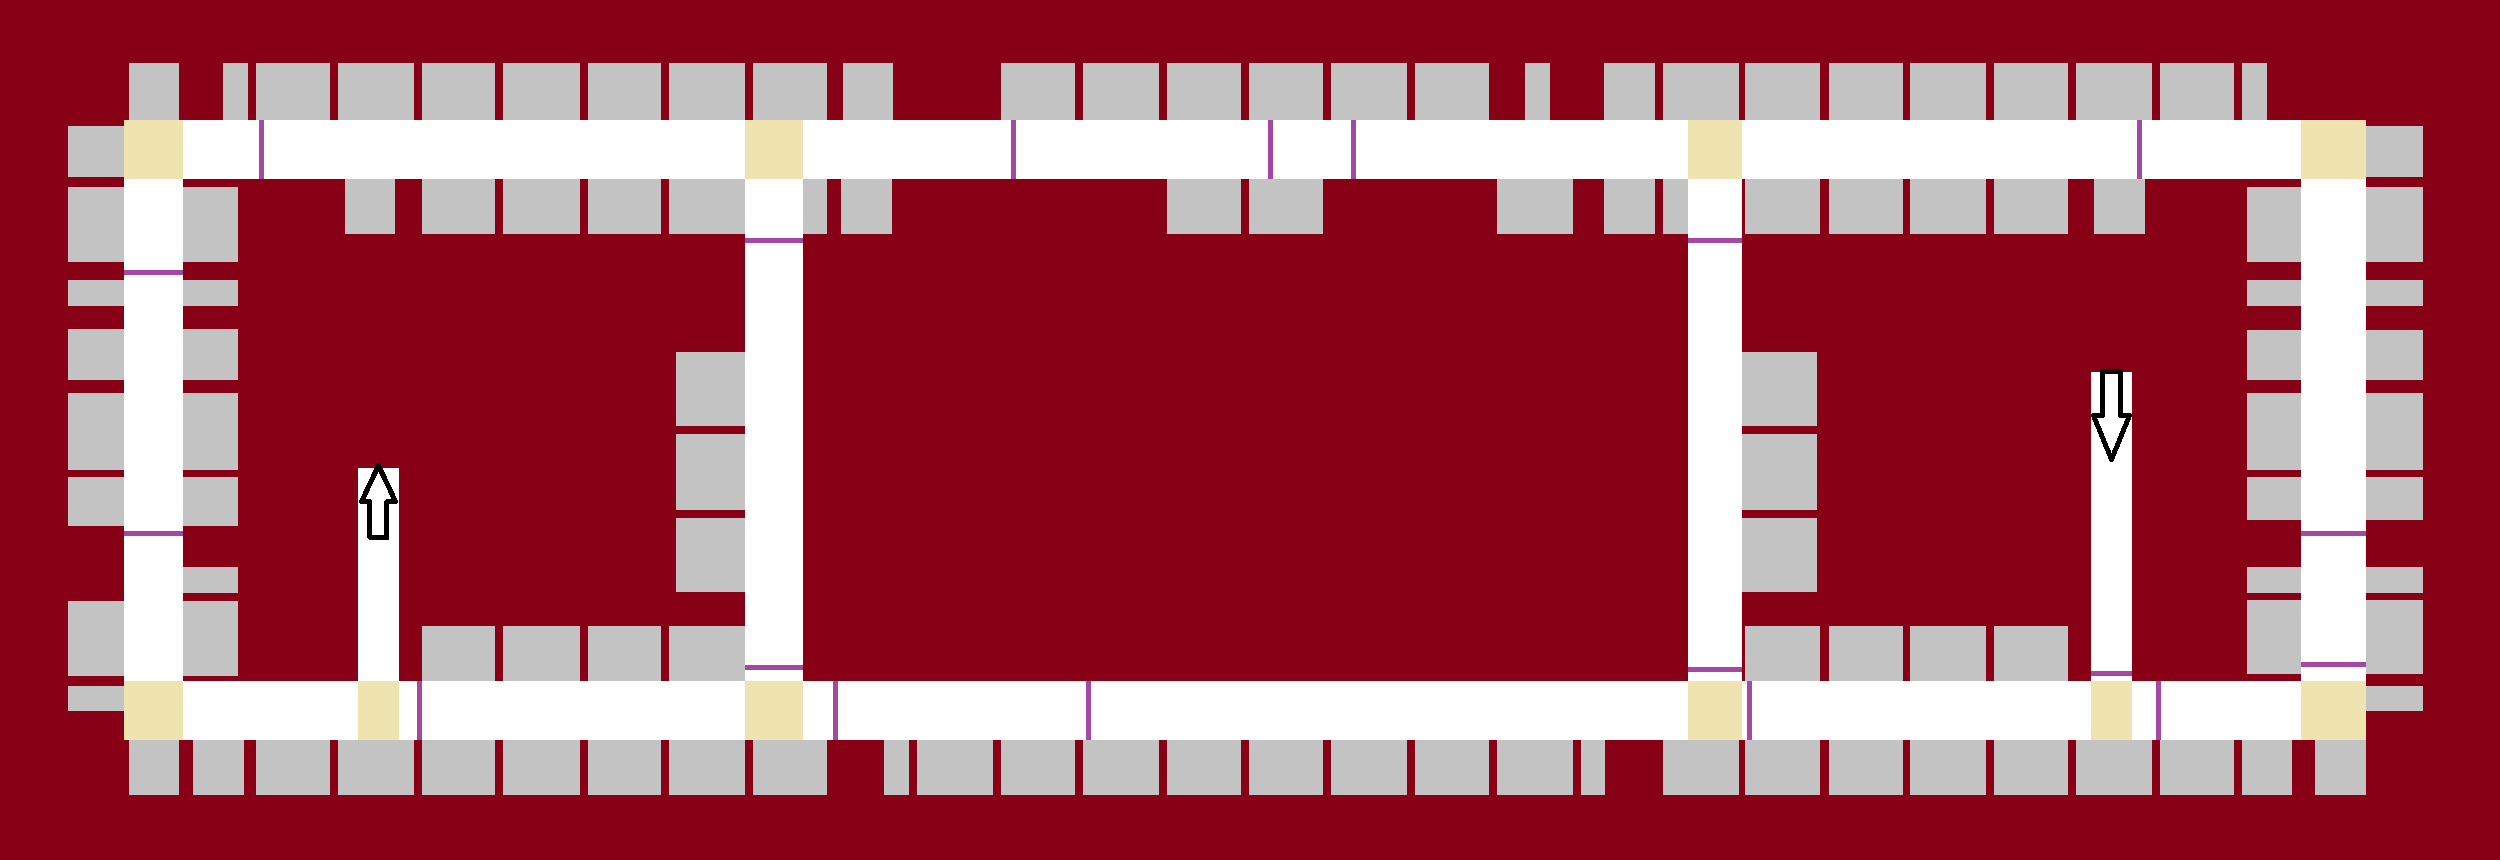
\includegraphics[scale=0.16]{map1}
        }
        \vfill
        \subfigure[] {
        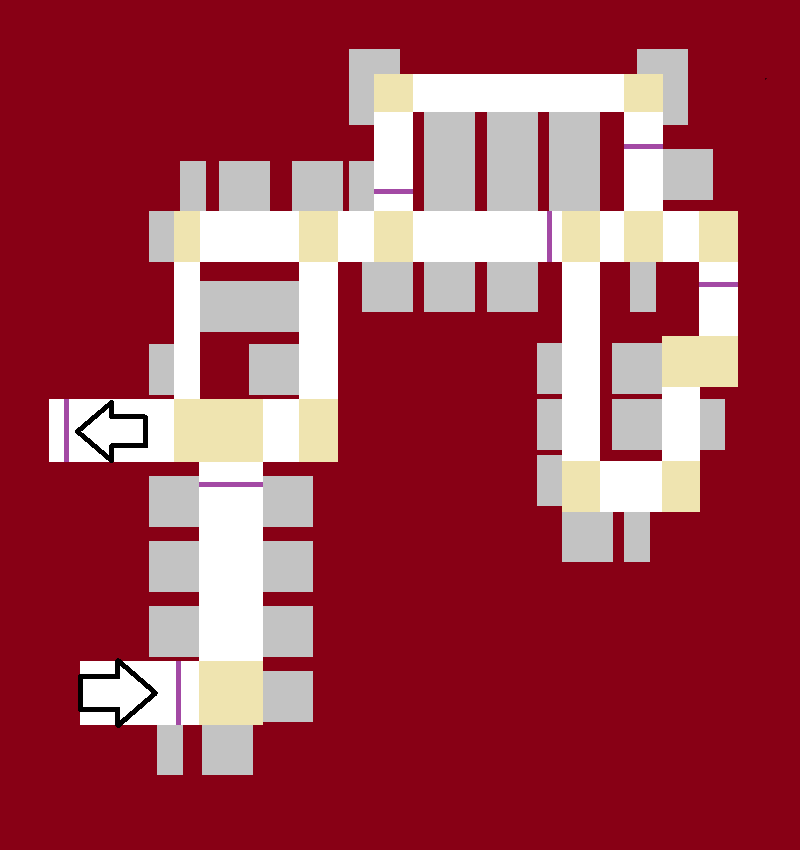
\includegraphics[scale=0.16]{map3}
        }
        \subfigure[] {
        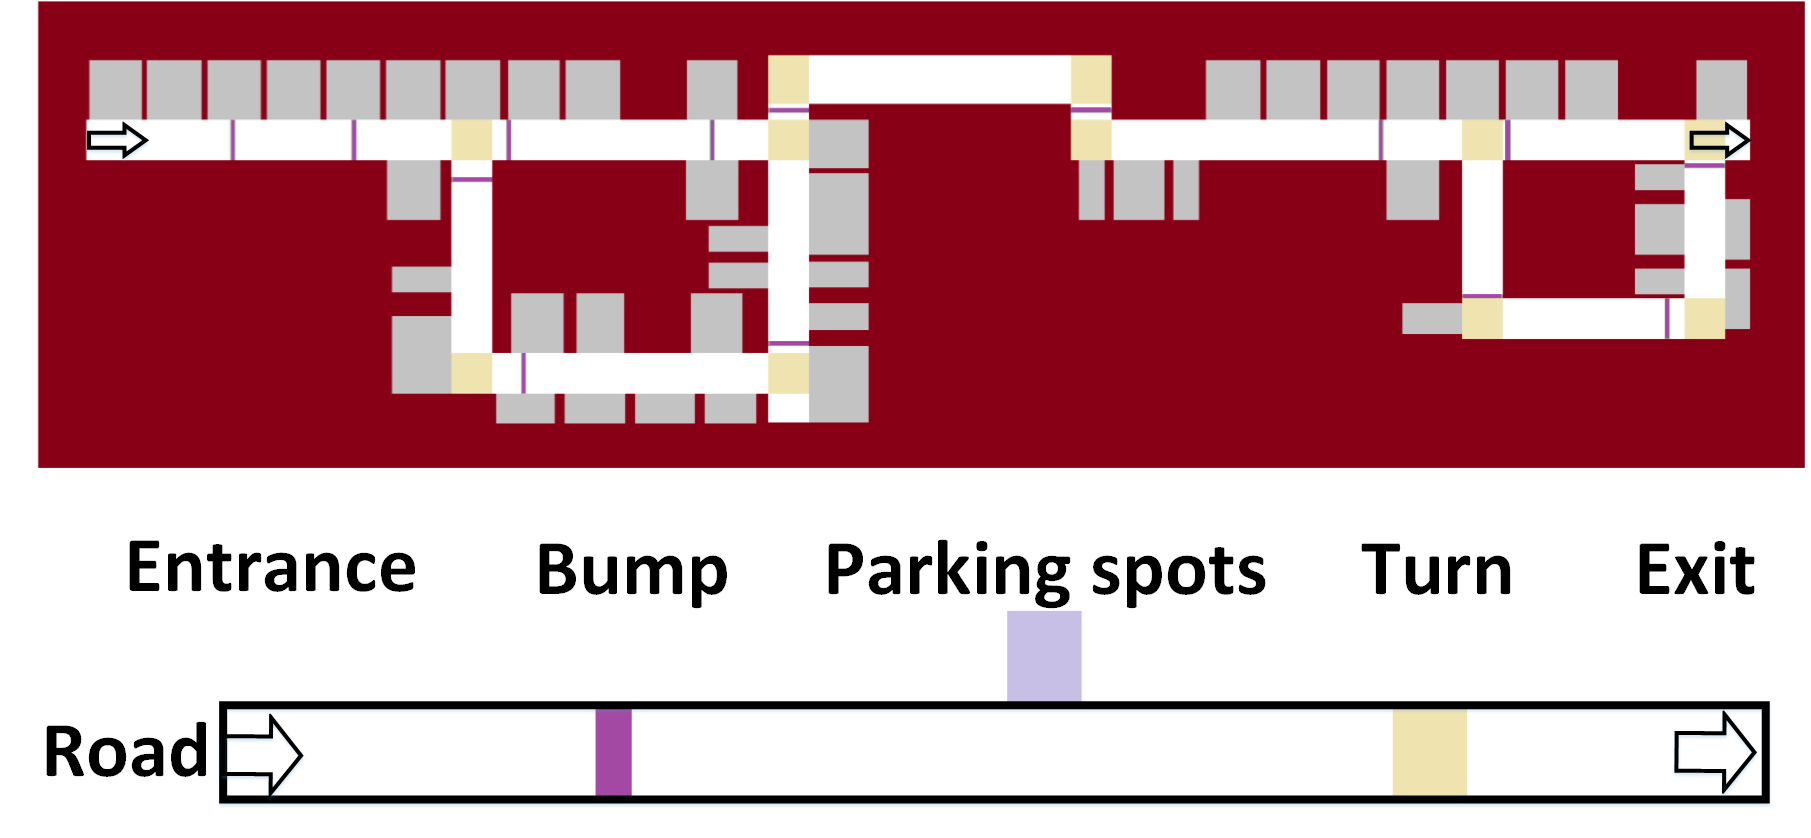
\includegraphics[scale=0.16]{map4}
        }
        \caption{Floor map of three underground parking lots: (a) parking lot 1: $250m\times 90m$ with 298 parking spots, 19 bumps and 10 turns. (b) parking lot 2: $80m\times 90m$ with 68 parking spots, 7 bumps and 14 turns. (c) parking lot 3: $180m\times 50m$ with 79 parking spots, 12 bumps and 11 turns. }\label{floorplan}
\end{figure*}

We use smartphones to collect motion sensor readings on a vehicle in three underground parking lots, and their size are $250m\times 90m$, $80m\times 90m$, and $180m\times 50m$, respectively. The floor plan of those three parking lots are shown in Figure~\ref{floorplan}. Each parking lot has one entrance and one exit, and there are 298, 68, 79 parking spots, 19, 7, 12 bumps, 10, 14, 11 turns and 4, 2, 2 slopes in each parking lot, respectively. During experiments, we conduct 20 vehicle traces in each parking lot with 4 iPhones with different poses to simultaneously collect inertial sensor data during the driving.
We design a mould to fix 4 iPhones with different poses as shown in Figure~\ref{pix:mould}. The mould is placed flat inside the vehicle with direction shown in Figure~\ref{pix:mould}.

As to evaluate our system's robustness, we invite three volunteers to drive their own cars in one parking lot, and their car's cost is around 10 thousand, 20 thousand and 30 thousand dollars, respectively.
During each driving, we start the data collection app developed by us on 4 phones to record their accelerometer and gyroscope readings before vehicle enters a parking lot, and ends app after vehicle stops at a parking spot.

We measure each pose's position in the mould as ground truth for the pose estimation algorithm.
The landmarks come across during the drive are recorded as ground truth for the landmark detection algorithm.
Also, the final position where the vehicle stops is recorded as ground truth for the localization algorithm.
\begin{figure}[h]
  \centering
  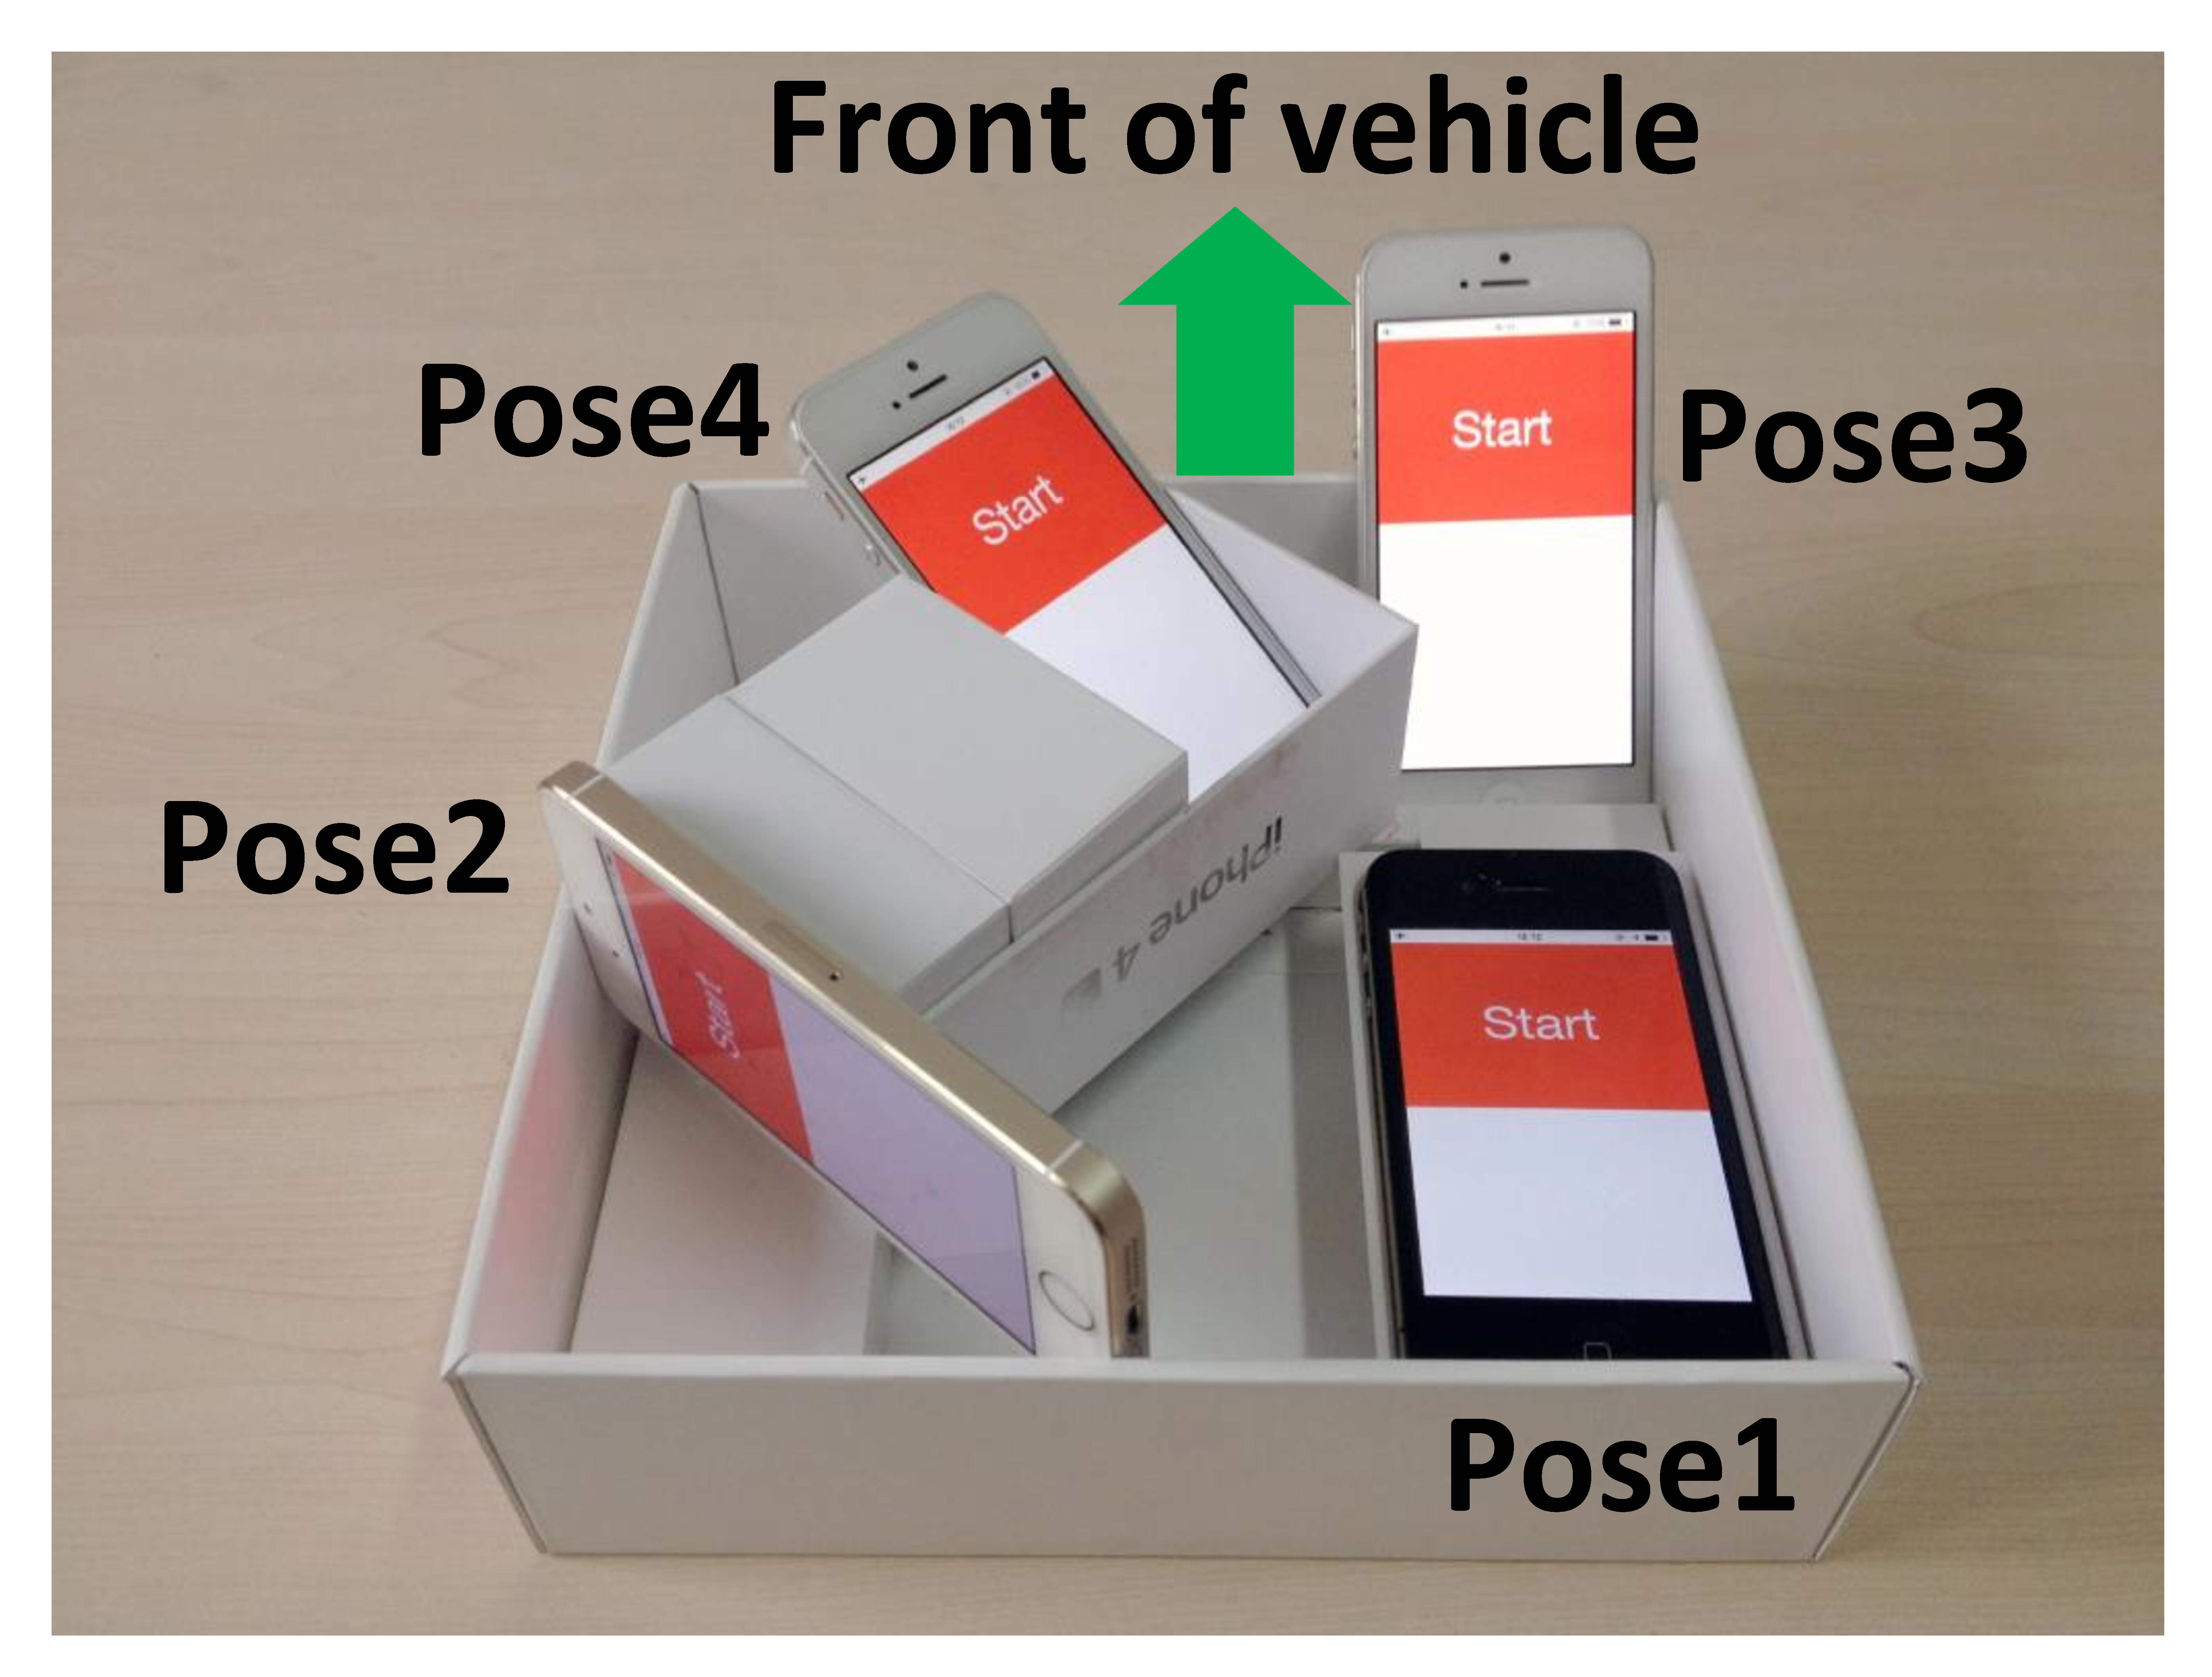
\includegraphics[width=0.48\textwidth]{mould.pdf}\\
  \vspace{5pt}
  \caption{Mould is with 4 iPhones. }\label{pix:mould}
\end{figure}

%We also realize our app in both iOS and Android development environments, and collect sensor readings on 6 phones with the same pose, i.e. iPhone 4S, iPhone 5, iPhone 5S, Samsung I9100, HTC G8 and Google Nexus 5.

\subsection{Evaluation of Pose Estimation}

Here we evaluate the performance of pose estimation algorithms, namely the accuracy of estimated smartphone's pose inside vehicle. We measure the orientation error between vehicle's estimated orientation and its ground truth orientation both in smartphone's coordinate system. We use the control variate method to evaluate the effect of different smartphone poses, driving styles and parking lots.

\begin{figure*}[t]
      \centering
      \vspace{-2pt}
        \subfigure[] {
        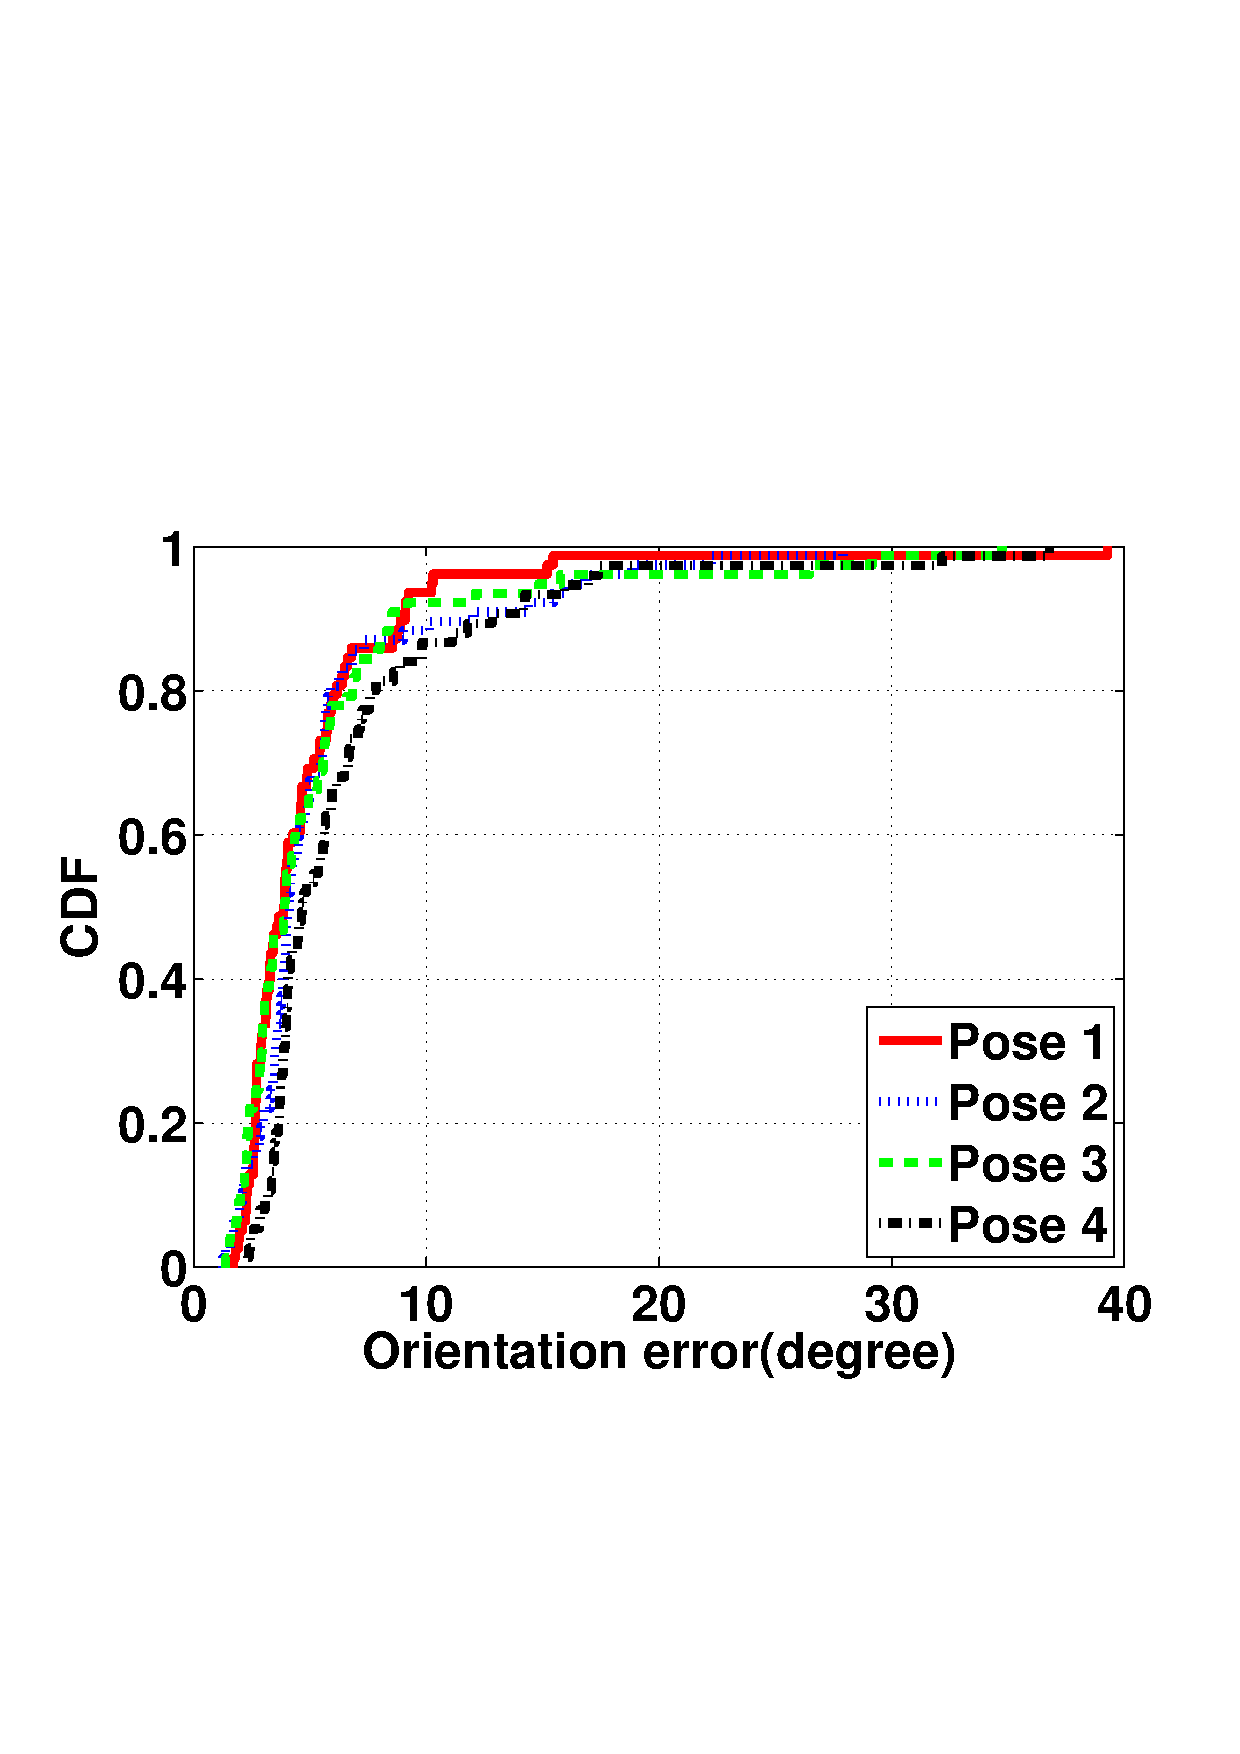
\includegraphics[width=2.2in]{pose}\label{pose}
        }
        \subfigure[] {
        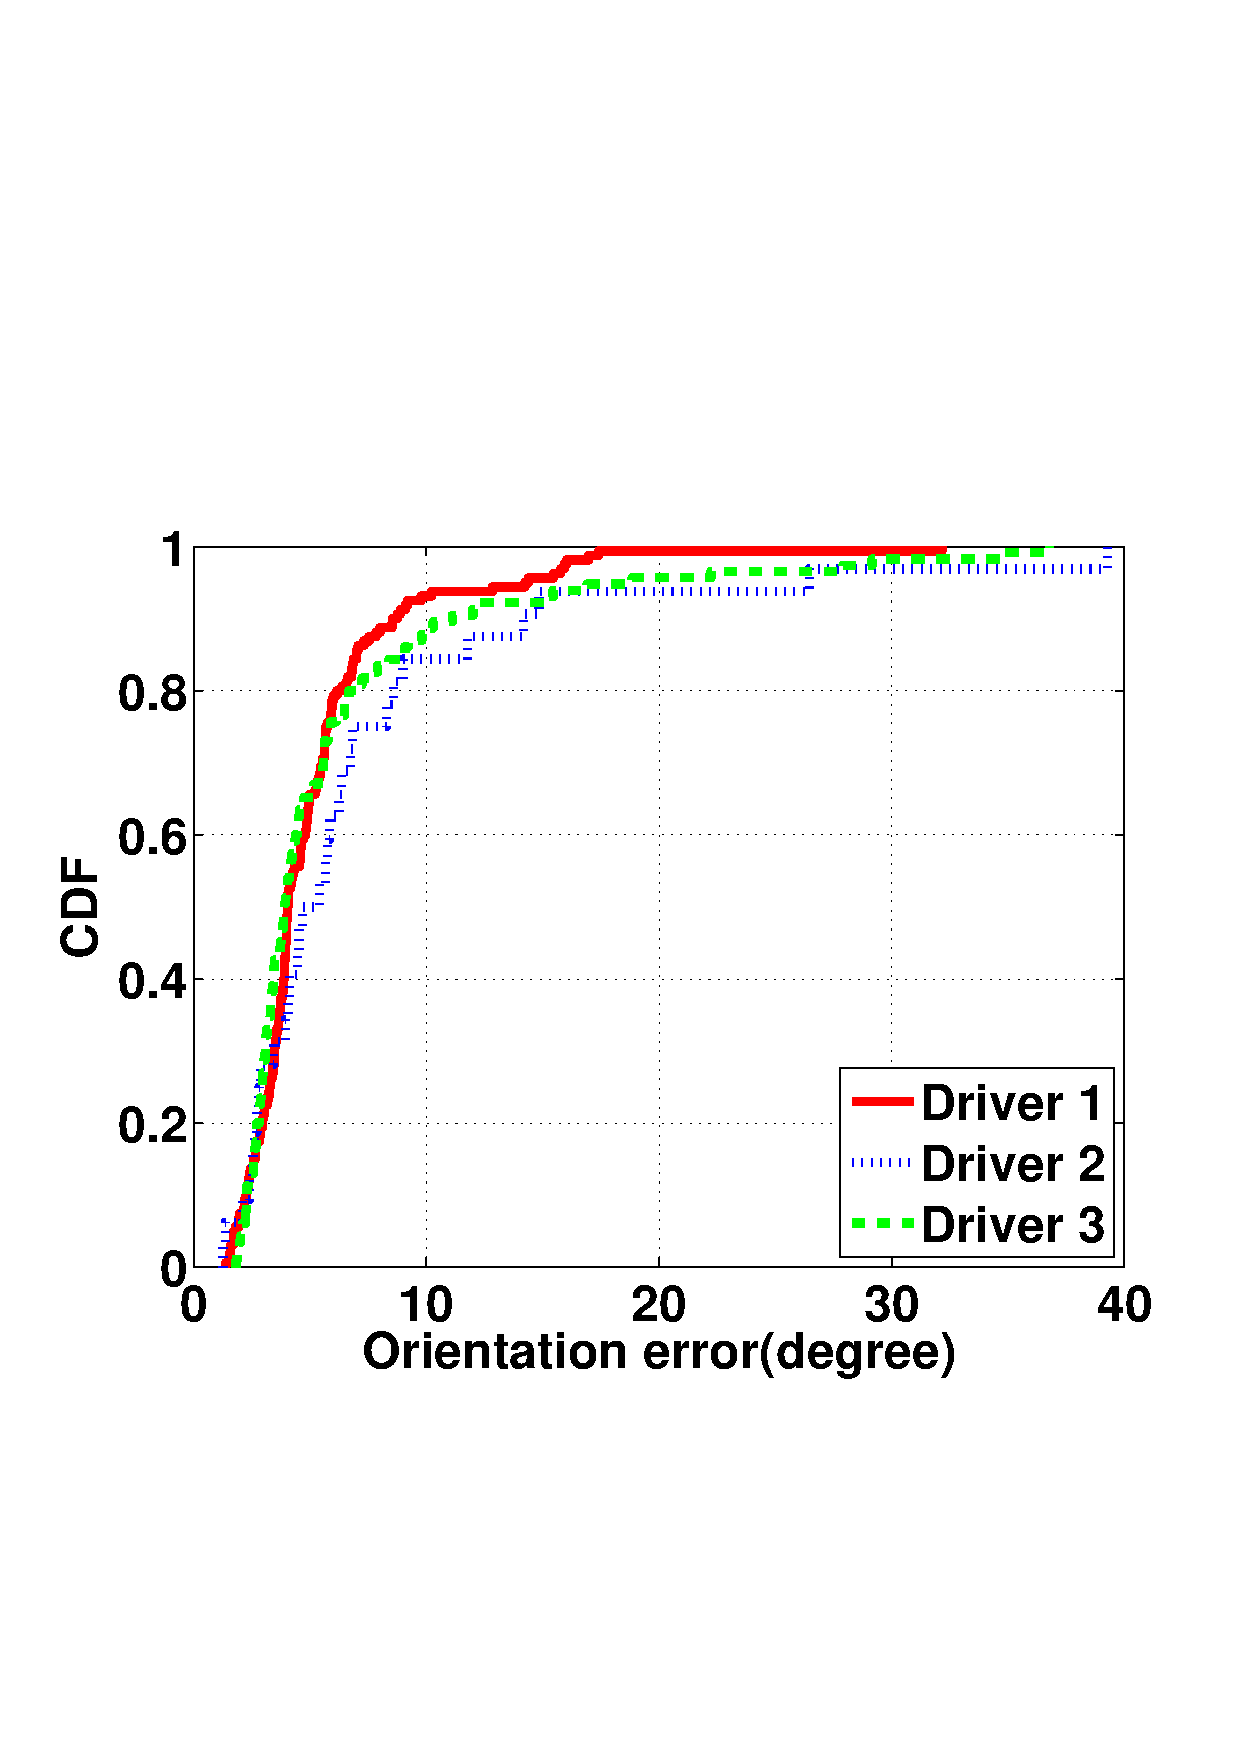
\includegraphics[width=2.2in]{style}\label{style}
        }
        \subfigure[] {
        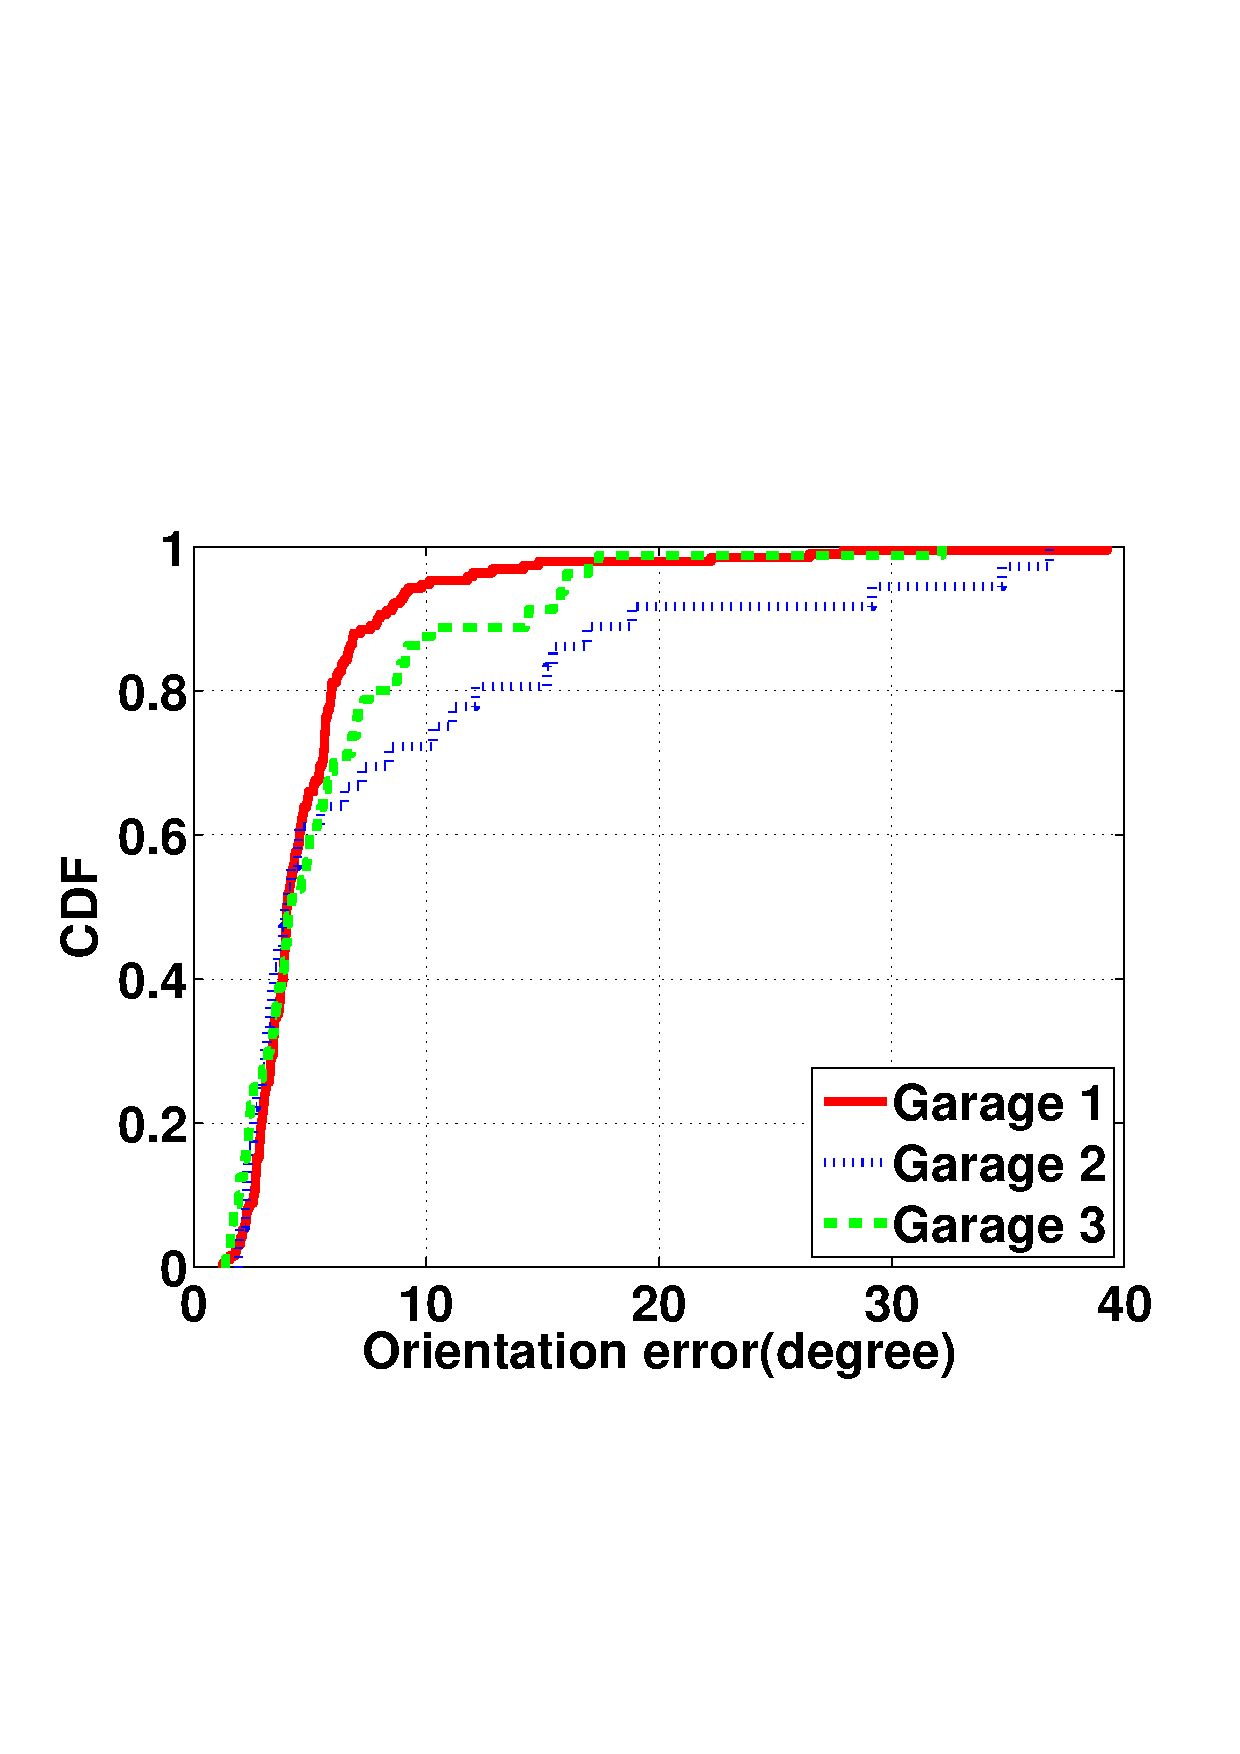
\includegraphics[width=2.2in]{place}\label{place}
        }
        \caption{Pose estimation error in different scenarios: (a) 4 different poses. (b) 3 different vehicles and drivers in one parking lot. (c) 3 different parking lots.}
\end{figure*}



Figure~\ref{pose} shows the orientation error with different smartphone poses. We could observe that the 90-percentile error is around 9 degrees, and the largest error is less than 40 degrees. Figure~\ref{style} presents the effect of driving styles, namely drivers, on our pose estimation. We could observe that despite different drivers and performance of cars, we achieve similar pose estimation accuracy, also around 9 degrees at 90-percentile. Figure~\ref{place} illustrates that our algorithm works well in different parking lots, they all achieve 13 degrees accuracy at 90-percentile, and Parking lot 2 has the largest error of 16 degrees, due to its short straight road which we use to compute the vehicle's orientation.

%The orientation of either smartphone or vehicle could be presented as a 3-dimension vector, thus we here use the cosine distance (cosine value of intersection angle between two vectors) to measure smartphone's pose, i.e. cosine distance between smartphone's vector and vehicle's vector. We also measure the ground truth smartphone's pose and then compute the cosine distance error in different scenarios.

%metric: cosine distance(for different pose, driving style, parking places).

In Section~3.4, we estimated the probability of the forward and backward directions of the vehicle, $p(\theta=\theta_2)$ and ${p(\theta=\theta_2)}$. And we also know which one is the real forward direction as we have recorded the ground truth. Then we can calculate the distribution of estimated probability of the backward direction,i.e., the estimation error. As showed in Figure~\ref{pix:direction_err}, it achieve more than 99\% accuracy at 90 percentile and a maximum error of 23\%.
\begin{figure}[h]
  \centering
  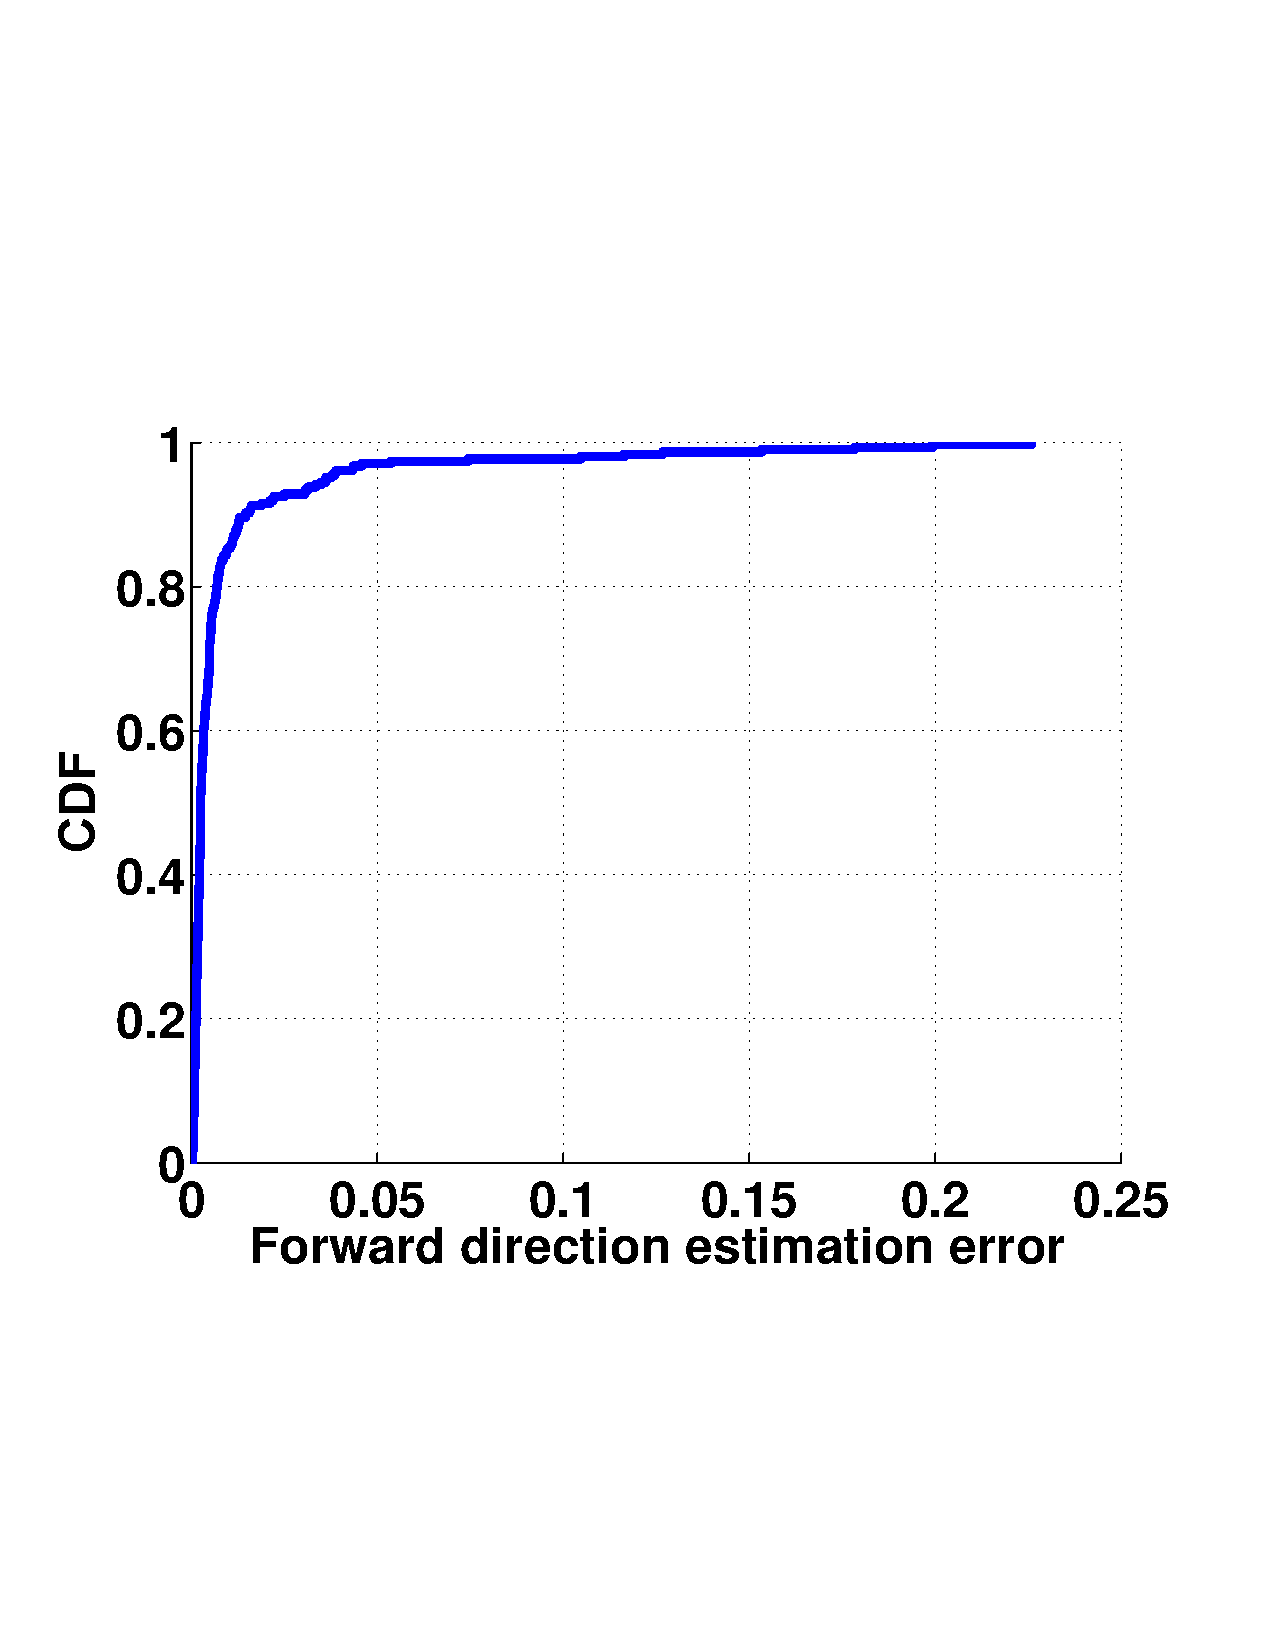
\includegraphics[width=0.42\textwidth]{direction_err}\\
  \caption{The distribution of estimated probability of the backward direction.}\label{pix:direction_err}
\end{figure}

\begin{figure}[h]
  \centering
  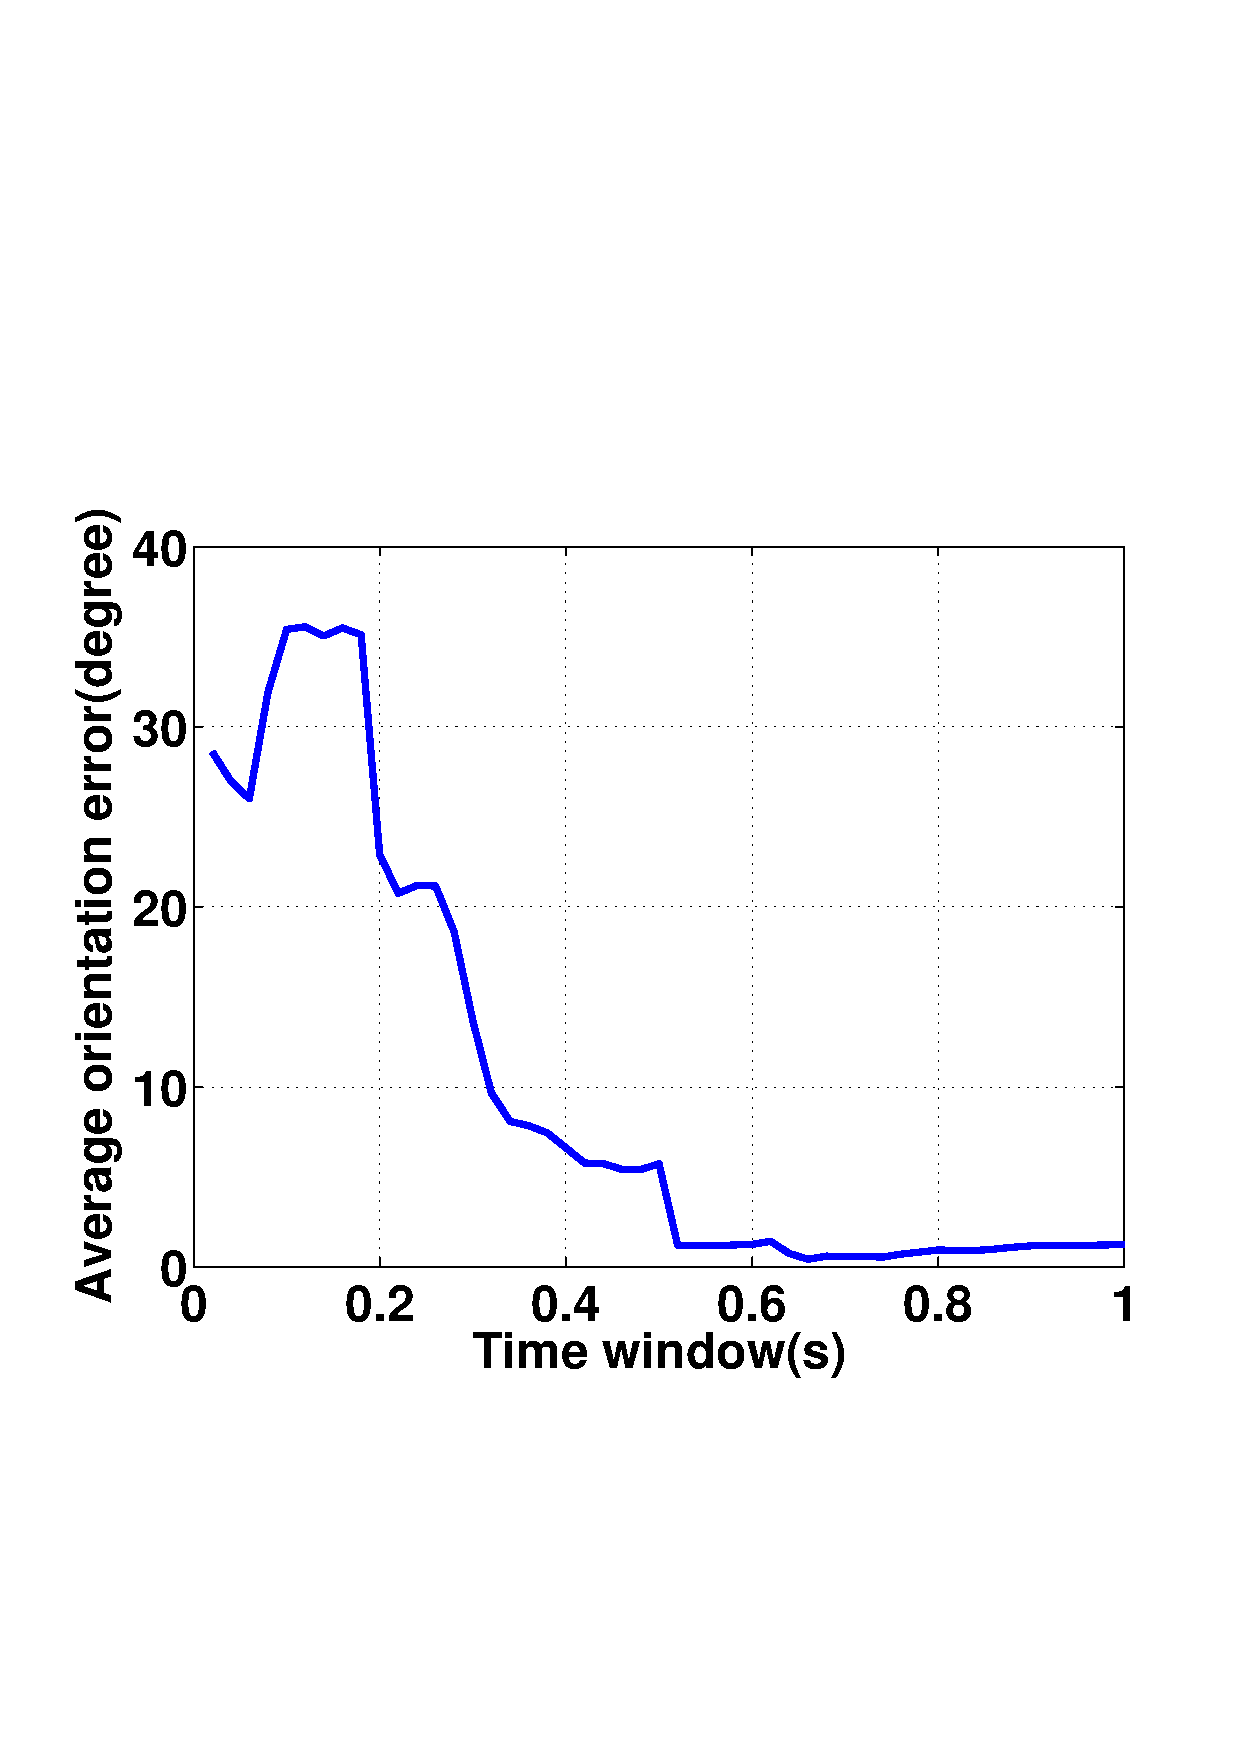
\includegraphics[width=0.42\textwidth]{time_pose}\\
  \caption{Orientation error of pose estimation for different time windows.}\label{pix:time_pose}
\end{figure}

Figure~\ref{pix:time_pose} shows the pose estimation accuracy with different time windows. We could see that the 90-percentile pose estimation error is reduced when increasing the time window for pose estimation algorithms. Additionally, the localization error stays stable when time window is larger than $0.5$s, which reflects realtime performance of our system.

\subsection{Evaluation of Landmark Detection}

Here we evaluate the performance of landmark detection using the precision and recall as metrics.
As to measure the precision and recall of landmark detection, we set breakpoints where a certain landmark is announced to be detected, and we check whether it corresponds to a correct landmark on the floor map at that time stamp. We also compute how many landmarks the vehicle goes through from floor map as its ground truth number of landmarks.

Since our calibration of vehicle localization mainly relies on the landmark detection, we prefer higher precision rather than recall. This is because if we omit a certain landmark, we'll just miss a chance for recalibration. On the contrary, the detection of a nonexistent landmark will lead our particles to somewhere unknown.

Table~\ref{tab:landmark_precision} shows the recall and precision for different landmarks. We observe that turn detection has detected all the turns correctly. Bump detecion has the lowest precision of $87$\%, and recall of $83$\%. This is because gyroscope sensor is much more precise than accelerometer sensor on smartphone, and there are many activities can be confused with bumps.

\begin{table}[!hbp]
\caption{Landmark detection performance for different landmarks}
\centering
\begin{tabular}{|c|c|c|c|}
\hline
 & Bump & Turn & Slope\\
\hline
Precision & 87\% & 100\% & 97\%\\
\hline
Recall & 83\% & 100\% & 95\%\\
\hline
\end{tabular}
\label{tab:landmark_precision}
\end{table}

Table~\ref{tab:pose_precision} shows the precisions with different poses of smartphone, we can observe that all precisions are quite high, while twos are relatively lower. This is because that in some positions, the smartphones are also sensitive to the jolting of the car, which may falsely be detected as a bump. Table~\ref{tab:style_precision} presents the effect of driving styles on our landmark detection. We achieve similar landmark detection precision, around $92$\%. Table~\ref{tab:place_precision} illustrates that we achieve quite different recall in different parking lots since the recall is effected by the property of landmarks.



\begin{table}[!hbp]
\caption{Performance of landmark detection with different poses}
\centering
\begin{tabular}{|c|c|c|c|c|}
\hline
 & Pose 1& Pose 2& Pose 3& Pose 4\\
\hline
Precision & 93\% & 88\% & 85\% & 93\%\\
\hline
Recall & 88\% & 89\% & 87\% & 85\%\\
\hline
\end{tabular}
\label{tab:pose_precision}
\end{table}


\begin{table}[!hbp]
\caption{Performance of landmark detection with different drivers}
\centering
\begin{tabular}{|c|c|c|c|}
\hline
 & Driver 1& Driver 2& Driver 3\\
\hline
Precision & 93\% & 92\% & 91\%\\
\hline
Recall & 89\% & 90\% & 87\%\\
\hline
\end{tabular}
\label{tab:style_precision}
\end{table}


\begin{table}[!hbp]
\caption{Performance of landmark detection with different garages}
\centering
\begin{tabular}{|c|c|c|c|}
\hline
 & Garage 1& Garage 2& Garage 3\\
\hline
Precision & 94\% & 90\% & 92\%\\
\hline
Recall & 78\% & 93\% & 91\%\\
\hline
\end{tabular}
\label{tab:place_precision}
\end{table}



\subsection{Evaluation of tracking}

\begin{figure*}[t]
      \centering
      \vspace{-2pt}
        \subfigure[] {
        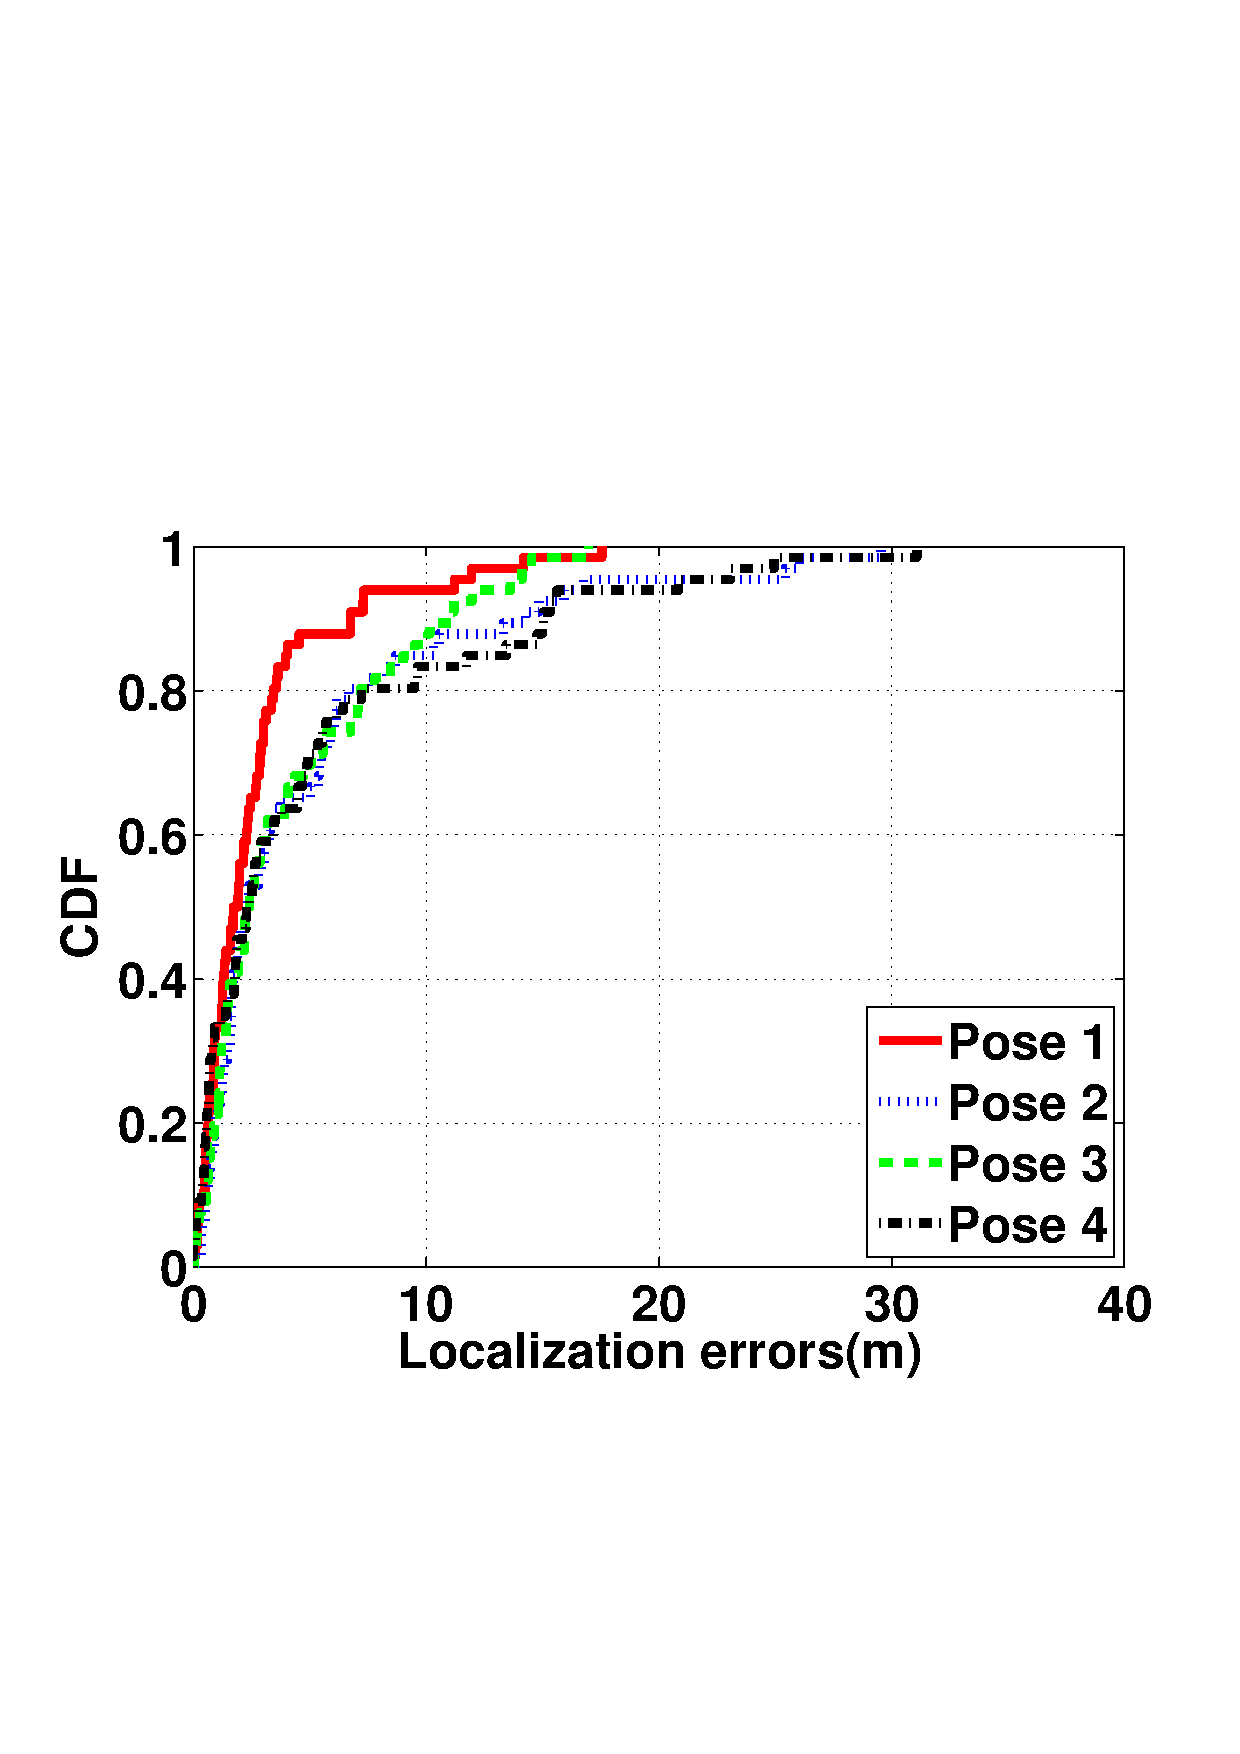
\includegraphics[width=2.2in]{err_pose}\label{err_pose}
        }
        \subfigure[] {
        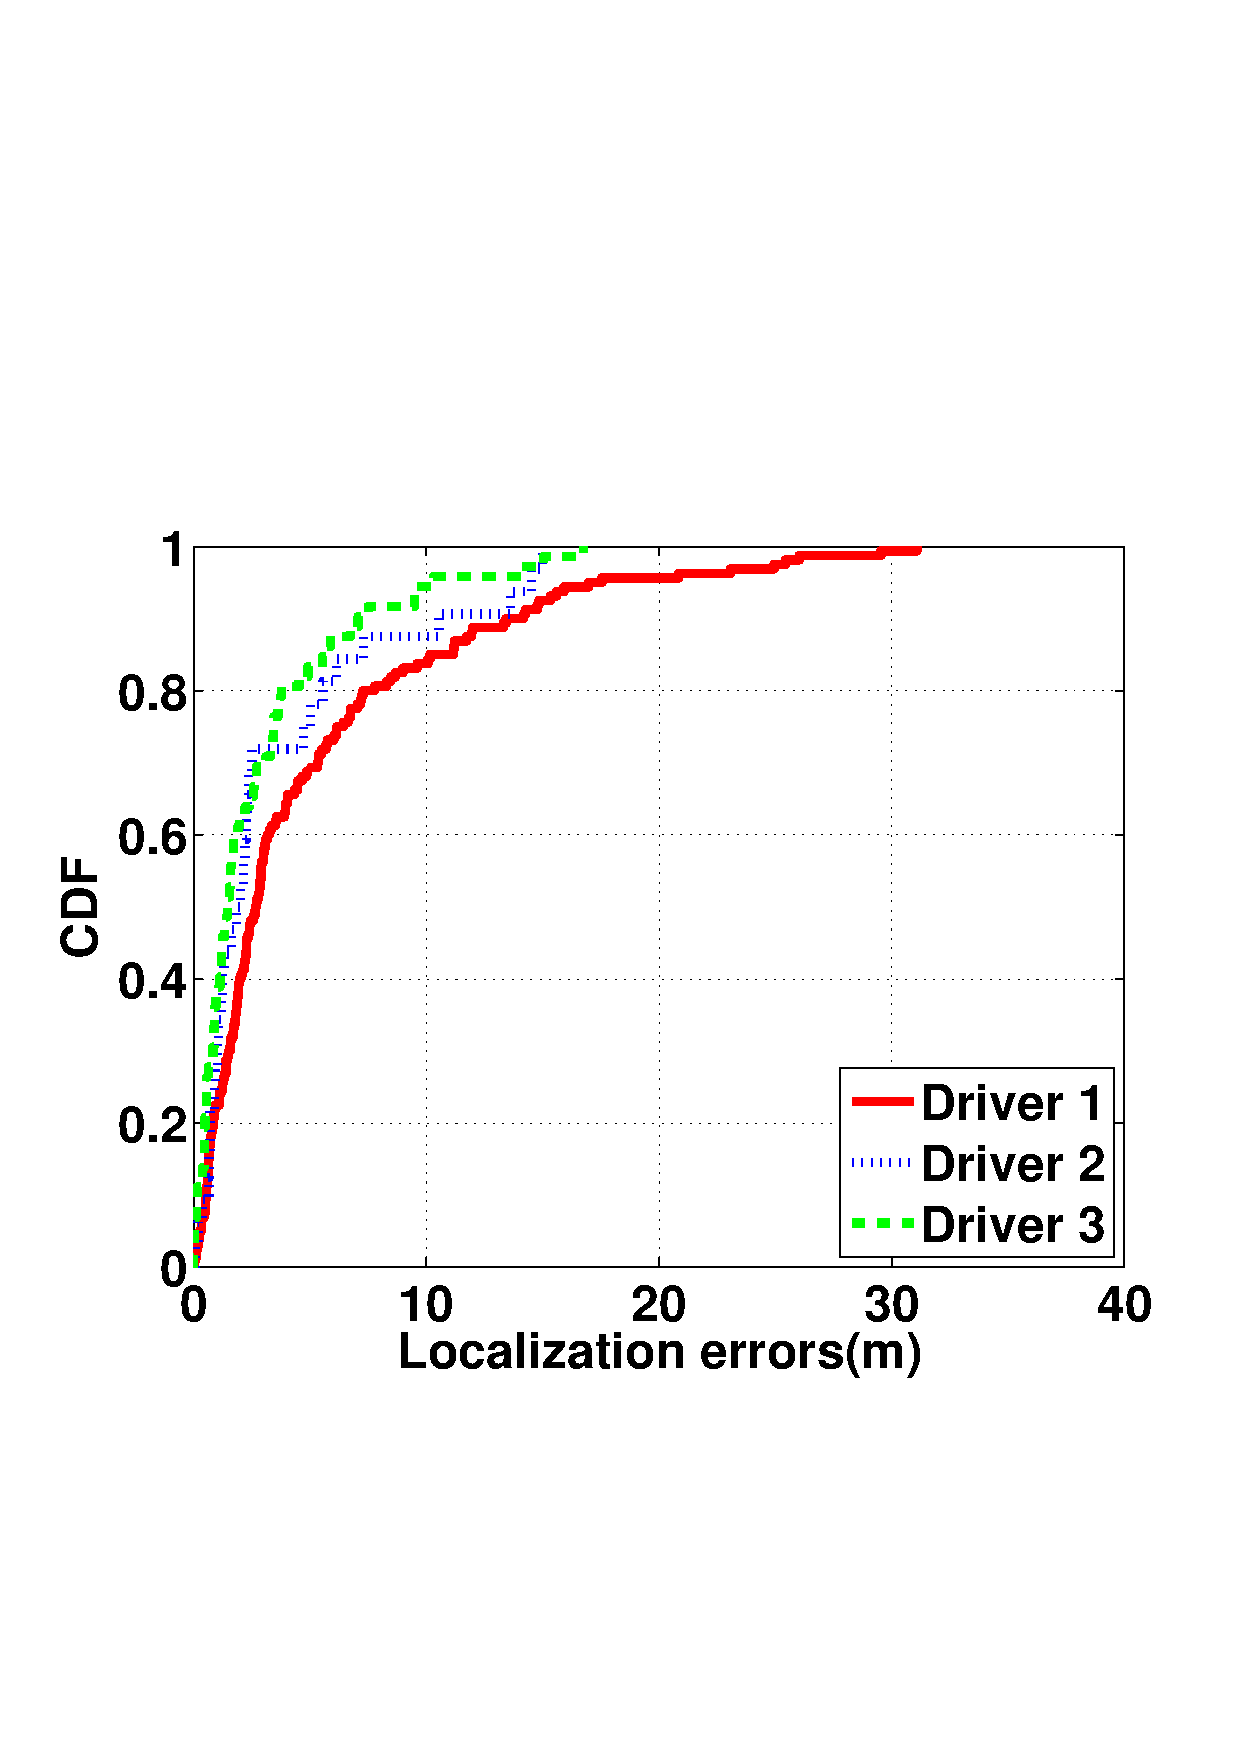
\includegraphics[width=2.2in]{err_style}\label{err_style}
        }
        \subfigure[] {
        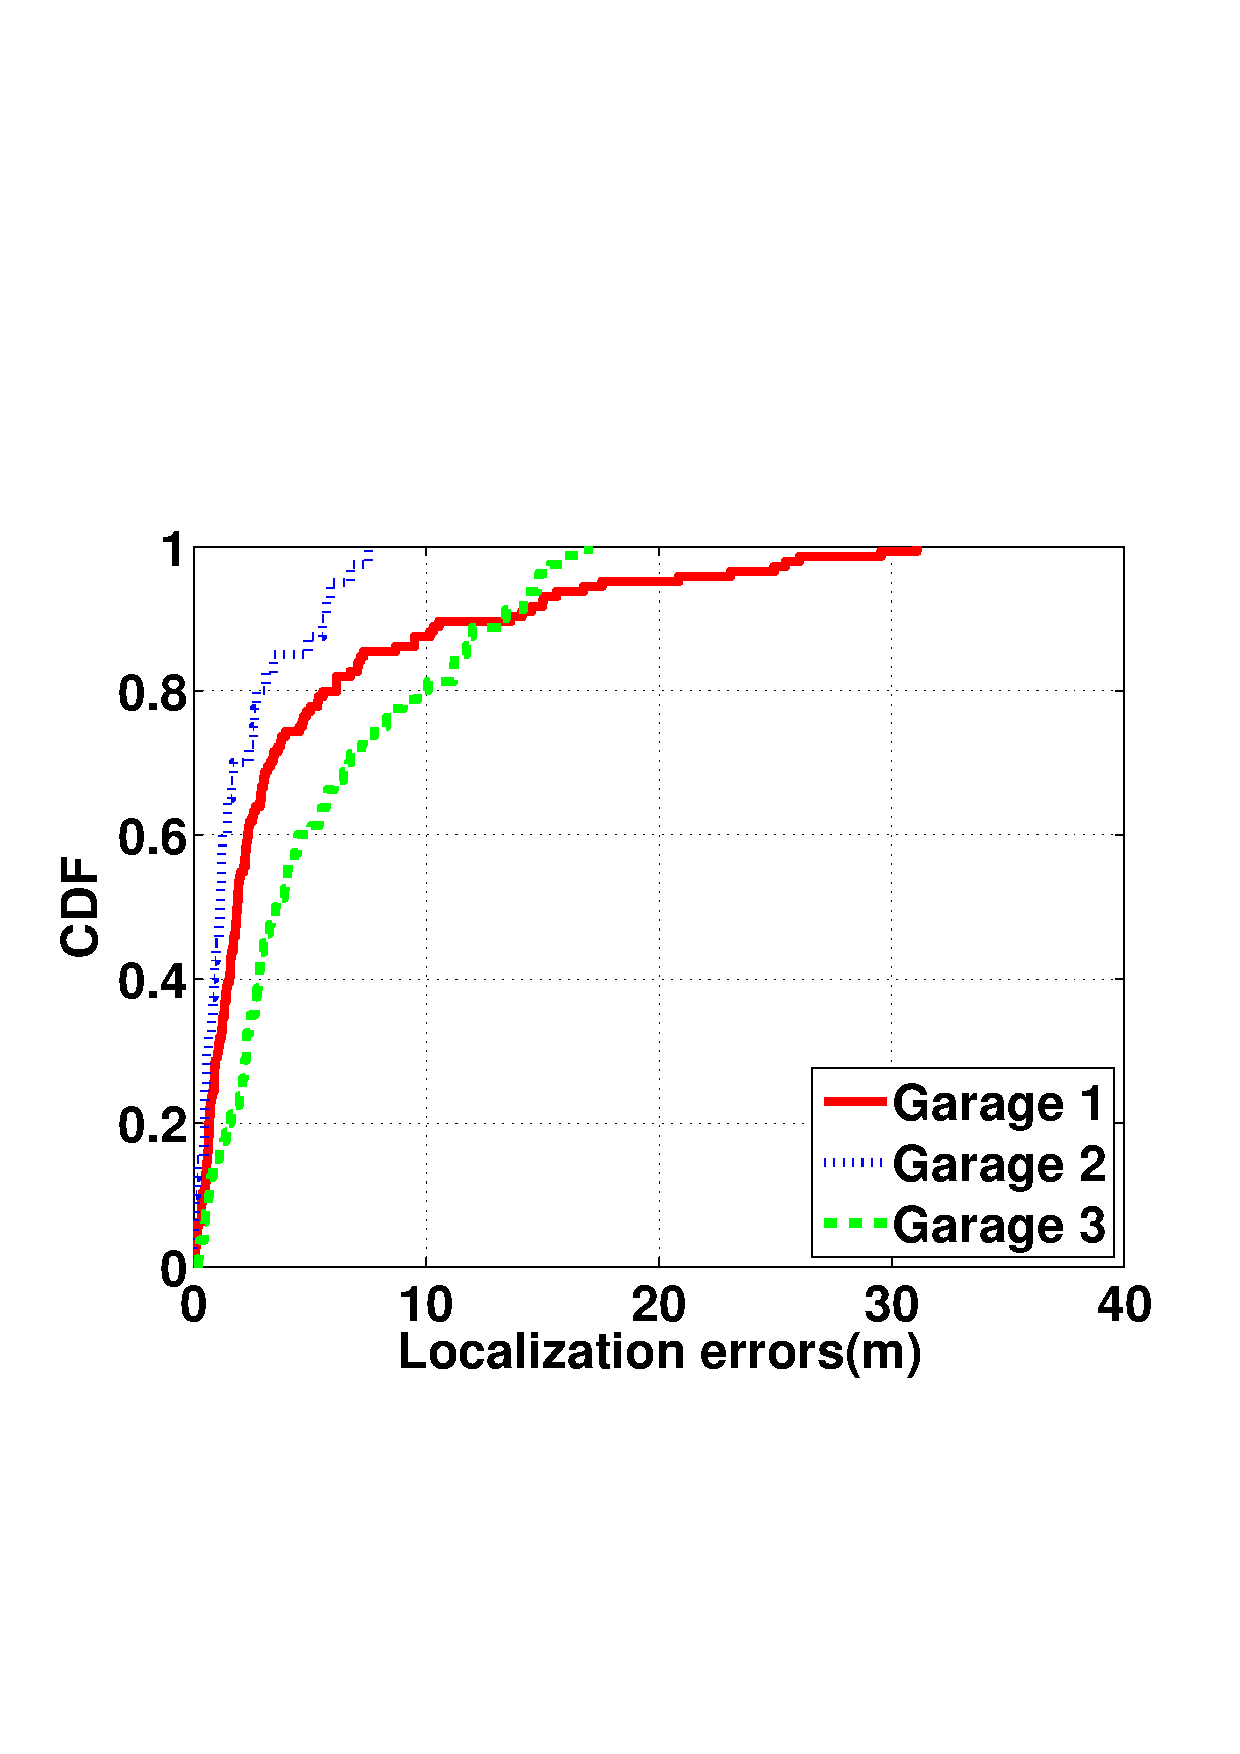
\includegraphics[width=2.2in]{err_place}\label{err_place}
        }
        \caption{Vehicle localization errors in different scenarios: (a) 4 different poses. (b) 3 different cars and drivers in one parking lot. (c) 3 different parking lots. }\label{locerr}
\end{figure*}

Figure~\ref{locerr} shows the vehicle localization accuracy in different scenarios. The 90-percentile localization error is around $10m$ for all 4 poses, and the maximum errors are about $30m$, shown in Figure~\ref{err_pose}.
Additionally, as Figure~\ref{err_style} shows, different drive styles achieve localization accuracy around $10m$ at 90-percentile.
Figure~\ref{err_place} shows the localization error in 3 parking lots, which are different since those parking lots have different shape and size.

%Localization error(for different pose, driving style, parking places).

%Error along time for three cases.


\begin{figure}[h]
  \centering
  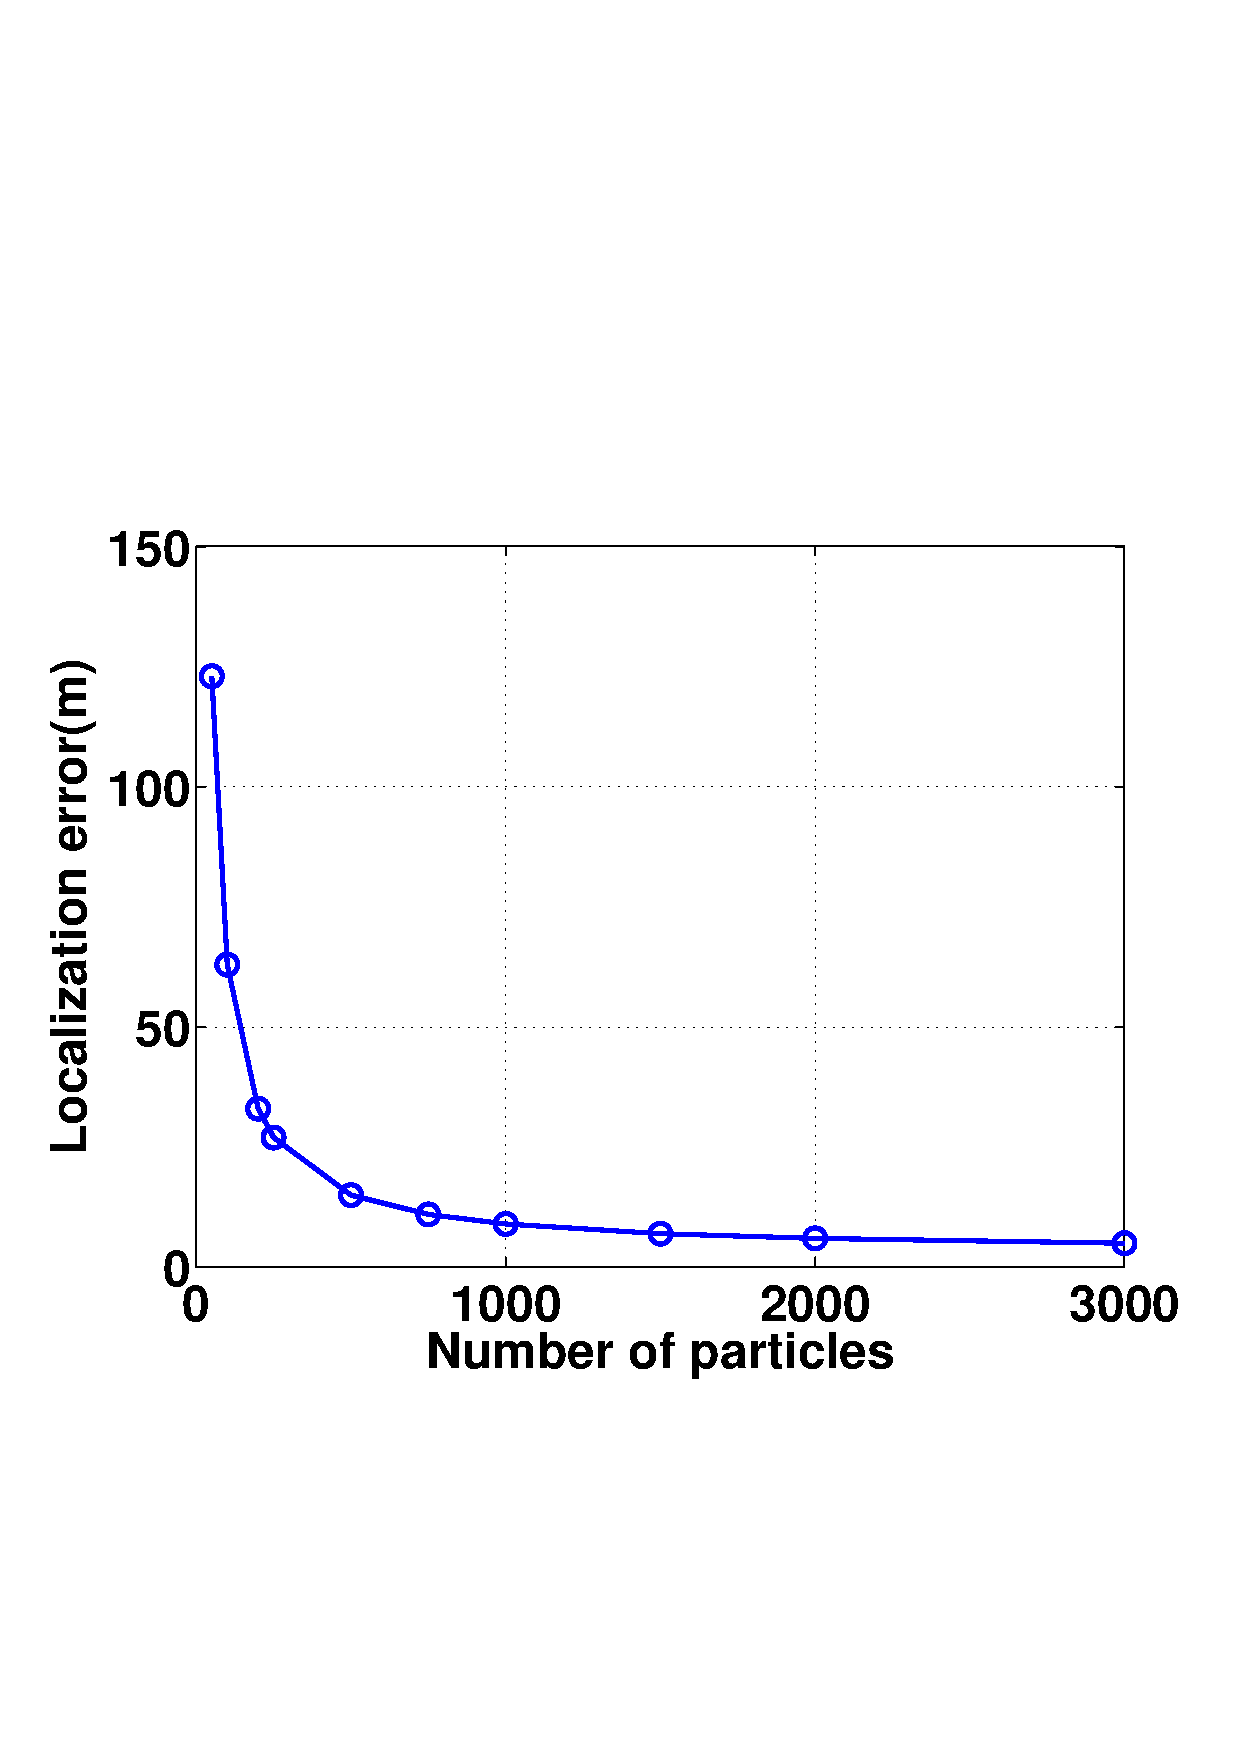
\includegraphics[width=0.48\textwidth]{particle_number}\\
  \caption{Performance of different particle numbers. }\label{pix:particle_number}
\end{figure}

Additionally, we evaluate the performance of the localization algorithm with different particle numbers.
As we can see in the Figure~\ref{pix:particle_number}, localization errors shrink along with the increasing particle number and almost converge when then its number exceeds a certain threshold, namely $2000$ particles.


%Error for different number of PF, real-time system.

%Finally, we implements our system on both iOS and Android development environments, and evaluate its performance on several types of  smartphones. Figure~\ref{} shows that iPhones generally have lower localization errors than Android phones by XX percentile. The major reason is possibly due to iPhones have more precise accelerometer and gyroscope sensors.

%Error for different devices.
